\documentclass[UTF8, a4paper]{report}
\usepackage[margin=0.5in]{geometry}
\usepackage{graphicx}
\usepackage{xetexko}

\title{%
    <컴퓨터프로그래밍 3> 실습 보고서 \\ 
    \large [제 08 주] 리스트 성능측정 1}
\author{201704150 허강준}
\date{\today}


\begin{document}
    \maketitle
    \tableofcontents

    \chapter{프로그램 설명서}
        본 보고서에서는 비정렬 리스트를 정의하고 여러 동작의 성능을 측정하는 프로그램에 대해 기술한다.

        \section{프로그램의 전체 설계 구조 (MVC 등)}
            
            \paragraph{%
                \normalfont 본 프로그램은 크게 프로그램의 제어를 담당하는 Controller인 \texttt{app\_controller}, 입/출력을 담당하는 View인 \texttt{app\_view}, 그리고 비정렬 리스트 모델인 \texttt{unsorted\_list}, 성능 측정 타이머 모델인 \texttt{perf\_timer}, 그리고 테스트 파라메터 관리를 위한 \texttt{parameter\_set}등으로 나뉜다. 또한 리스트 처리를 위하여 C++의 Standard Template Library에 정의된 \texttt{vector} Type을 지난 과제에서 가져왔다.
            }
            
        \section{함수 설명서}
            
            \paragraph{\texttt{VECTOR(type)}}
            \paragraph{%
                \normalfont C++의 Standard Template Library에 정의된 Container Template Type인 \texttt{vector}를 일부 구현하였다. 구현된 메서드는 \texttt{new},  \texttt{delete}, \texttt{at}, \texttt{front}, \texttt{back}, \texttt{data}, \texttt{empty}, \texttt{size}, \texttt{max\_size}, \texttt{clear}, \texttt{insert}, \texttt{erase}, \texttt{push\_back}, \texttt{pop\_back}, \texttt{swap} 이다.
            }

            \paragraph{\texttt{parameter\_set\_new}}
            \paragraph{%
                \normalfont 파라메터 세트 생성자
            }

            \paragraph{\texttt{parameter\_set\_new\_with}}
            \paragraph{%
                \normalfont 최소 테스트 케이스 수, 최대, 증가 수를 인자로 받는 parameter\_set 생성자
            }

            \paragraph{\texttt{parameter\_set\_delete}}
            \paragraph{%
                \normalfont 파라메터 세트 소멸자
            }

            \paragraph{\texttt{parameter\_set\_set\_min\_test\_size}}
            \paragraph{%
                \normalfont 최소 테스트 케이스 수를 설정
            }

            \paragraph{\texttt{parameter\_set\_get\_min\_test\_size}}
            \paragraph{%
                \normalfont 최소 테스트 케이스 수를 반환
            }

            \paragraph{\texttt{parameter\_set\_set\_interval\_size}}
            \paragraph{%
                \normalfont 테스트 케이스 증가 수를 설정
            }

            \paragraph{\texttt{parameter\_set\_get\_interval\_size}}
            \paragraph{%
                \normalfont 테스트 케이스 증가 수를 반환
            }

            \paragraph{\texttt{parameter\_set\_set\_number\_of\_tests\_size}}
            \paragraph{%
                \normalfont 총 테스트 수 설정
            }

            \paragraph{\texttt{parameter\_set\_get\_number\_of\_tests\_size}}
            \paragraph{%
                \normalfont 총 테스트 수를 반환
            }

            \paragraph{\texttt{parameter\_set\_max\_test\_size}}
            \paragraph{%
                \normalfont 입력된 최소 테스트 케이스 수 및 증가 수, 총 테스트 수를 이용하여 최대 테스트 케이스 수를 반환
            }

            \paragraph{\texttt{perf\_timer\_new}}
            \paragraph{%
                \normalfont 타이머 생성자
            }

            \paragraph{\texttt{perf\_timer\_delete}}
            \paragraph{%
                \normalfont 타이머 소멸자
            }

            \paragraph{\texttt{perf\_timer\_start}}
            \paragraph{%
                \normalfont 타이머 시작
            }

            \paragraph{\texttt{perf\_timer\_stop}}
            \paragraph{%
                \normalfont 타이머 종료
            }

            \paragraph{\texttt{perf\_timer\_duration}}
            \paragraph{%
                \normalfont 측정된 시간 반환
            }

            \paragraph{\texttt{appview\_out}}
            \paragraph{%
                \normalfont 문자열 출력 및 개행
            }

            \paragraph{\texttt{app\_controller\_init\_performance\_measurement}}
            \paragraph{%
                \normalfont \texttt{parameter\_set}에서 관리할 최소 테스트 케이스 수, 증가 수, 총 테스트 수를 초기화
            }

            \paragraph{\texttt{app\_controller\_create}}
            \paragraph{%
                \normalfont 컨트롤러 생성자
            }

            \paragraph{\texttt{app\_controller\_time\_for\_unsorted\_array\_list\_remove\_max}}
            \paragraph{%
                \normalfont 최대값 삭제 테스트를 수행하고 수행 시간을 반환
            }
            
            \paragraph{\texttt{app\_controller\_time\_for\_unsorted\_array\_list\_add}}
            \paragraph{%
                \normalfont 리스트 추가 테스트를 수행하고 수행 시간을 반환
            }
            
            \paragraph{\texttt{app\_controller\_generate\_test\_data\_by\_random\_numbers}}
            \paragraph{%
                \normalfont 현재 시간을 기반으로 한 유사랜덤 테스트 데이터를 생성
            }
            
            \paragraph{\texttt{app\_controller\_show\_results}}
            \paragraph{%
                \normalfont 측정 결과를 출력
            }
            
            \paragraph{\texttt{app\_controller\_run}}
            \paragraph{%
                \normalfont 프로그램 메인 루틴 정의
            }
            
            \paragraph{\texttt{app\_controller\_delete}}
            \paragraph{%
                \normalfont 컨트롤러 소멸자
            }
            
            \paragraph{\texttt{unsorted\_list\_remove\_max}}
            \paragraph{%
                \normalfont 최댓값을 리스트에서 제거하는 함수 
            }

            \paragraph{\texttt{unsorted\_list\_max\_position\_recursively}}
            \paragraph{%
                \normalfont 최댓값의 인덱스를 재귀적으로 찾는 함수
            }

        \section{종합 설명서}

            \paragraph{%
                \normalfont 이번 프로그램은 지난 마방진 성능 테스트 프로그램과 유사하게 성능 측정용 타이머를 사용한다. \texttt{Vector} 타입을 이용하여 비정렬 리스트를 구현하고, 해당 리스트에 대하여 테스트 케이스 별로 각각 삽입 및 최댓값 삭제 시간을 측정한다. 
            }
            
    \chapter{프로그램 장단점/특이점 분석}
            \section{비정렬 리스트의 특성}
            \paragraph{%
                \normalfont 비정렬 리스트는 내부 데이터의 정렬상태를 보장하지 않는다. 따라서, 현재 원소에 대해 이전 원소 혹은 다음 원소의 대소관계를 명확하게 정의하기 어렵다. 그러나 이러한 특성 덕에 삽입연산(맨 끝)시 \texttt{O(1)} 복잡도를 달성할 수 있다는 장점이 있다.
            }   

            \section{Windows vs POSIX \texttt{clock()}}
            \paragraph{%
                \normalfont \texttt{clock()}함수는 표준 C 라이브러리에 정의된 표준 함수이지만, Windows와 POSIX계열 운영체제간의 구현이 다르다. 특히 정밀도에서 차이가 나기 때문에 Windows의 경우 milisecond 이하의 단위의 정밀도를 확보하기가 어렵다. 따라서 Windows API에서 정의하는 \texttt{QueryPerformanceCounter}를 사용하여 CPU Timer Register를 참조하여 정밀한 CPU Time을 확보하여 성능측정에 이용할 수 있다.
            }

    \chapter{실행 결과 분석}
        \section{실행 결과 캡쳐}
        \begin{figure}[!htb]
            \centering
            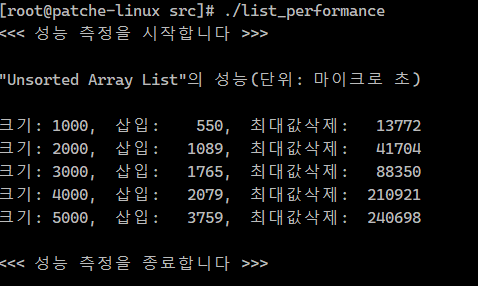
\includegraphics[width=\textwidth]{result.PNG}
            \caption{실행 결과1}
        \end{figure}
        
        \newpage

        \section{입력과 출력}
            실습 자료에서 제시된 테스트 데이터 생성 방법을 이용하였으며 출력 결과는 상기한 것과 같았음.
        \section{결과 분석}
            모든 입력에 대하여 정상적인 출력을 확인하였음.

    \chapter{소스코드}
        소스코드는 제출된 압축파일에 같이 동봉되어있으며 GitHub (0x00000FF/CNUCSE-Computer-Programming-III-2020-Spring) 에서도 열람할 수 있다.
\end{document}